\documentclass[]{article}
\usepackage{lmodern}
\usepackage{amssymb,amsmath}
\usepackage{ifxetex,ifluatex}
\usepackage{fixltx2e} % provides \textsubscript
\ifnum 0\ifxetex 1\fi\ifluatex 1\fi=0 % if pdftex
  \usepackage[T1]{fontenc}
  \usepackage[utf8]{inputenc}
\else % if luatex or xelatex
  \ifxetex
    \usepackage{mathspec}
  \else
    \usepackage{fontspec}
  \fi
  \defaultfontfeatures{Ligatures=TeX,Scale=MatchLowercase}
\fi
% use upquote if available, for straight quotes in verbatim environments
\IfFileExists{upquote.sty}{\usepackage{upquote}}{}
% use microtype if available
\IfFileExists{microtype.sty}{%
\usepackage{microtype}
\UseMicrotypeSet[protrusion]{basicmath} % disable protrusion for tt fonts
}{}
\usepackage[margin=1in]{geometry}
\usepackage{hyperref}
\hypersetup{unicode=true,
            pdftitle={Homework 1},
            pdfauthor={Christophe Hunt},
            pdfborder={0 0 0},
            breaklinks=true}
\urlstyle{same}  % don't use monospace font for urls
\usepackage{color}
\usepackage{fancyvrb}
\newcommand{\VerbBar}{|}
\newcommand{\VERB}{\Verb[commandchars=\\\{\}]}
\DefineVerbatimEnvironment{Highlighting}{Verbatim}{commandchars=\\\{\}}
% Add ',fontsize=\small' for more characters per line
\usepackage{framed}
\definecolor{shadecolor}{RGB}{248,248,248}
\newenvironment{Shaded}{\begin{snugshade}}{\end{snugshade}}
\newcommand{\KeywordTok}[1]{\textcolor[rgb]{0.13,0.29,0.53}{\textbf{{#1}}}}
\newcommand{\DataTypeTok}[1]{\textcolor[rgb]{0.13,0.29,0.53}{{#1}}}
\newcommand{\DecValTok}[1]{\textcolor[rgb]{0.00,0.00,0.81}{{#1}}}
\newcommand{\BaseNTok}[1]{\textcolor[rgb]{0.00,0.00,0.81}{{#1}}}
\newcommand{\FloatTok}[1]{\textcolor[rgb]{0.00,0.00,0.81}{{#1}}}
\newcommand{\ConstantTok}[1]{\textcolor[rgb]{0.00,0.00,0.00}{{#1}}}
\newcommand{\CharTok}[1]{\textcolor[rgb]{0.31,0.60,0.02}{{#1}}}
\newcommand{\SpecialCharTok}[1]{\textcolor[rgb]{0.00,0.00,0.00}{{#1}}}
\newcommand{\StringTok}[1]{\textcolor[rgb]{0.31,0.60,0.02}{{#1}}}
\newcommand{\VerbatimStringTok}[1]{\textcolor[rgb]{0.31,0.60,0.02}{{#1}}}
\newcommand{\SpecialStringTok}[1]{\textcolor[rgb]{0.31,0.60,0.02}{{#1}}}
\newcommand{\ImportTok}[1]{{#1}}
\newcommand{\CommentTok}[1]{\textcolor[rgb]{0.56,0.35,0.01}{\textit{{#1}}}}
\newcommand{\DocumentationTok}[1]{\textcolor[rgb]{0.56,0.35,0.01}{\textbf{\textit{{#1}}}}}
\newcommand{\AnnotationTok}[1]{\textcolor[rgb]{0.56,0.35,0.01}{\textbf{\textit{{#1}}}}}
\newcommand{\CommentVarTok}[1]{\textcolor[rgb]{0.56,0.35,0.01}{\textbf{\textit{{#1}}}}}
\newcommand{\OtherTok}[1]{\textcolor[rgb]{0.56,0.35,0.01}{{#1}}}
\newcommand{\FunctionTok}[1]{\textcolor[rgb]{0.00,0.00,0.00}{{#1}}}
\newcommand{\VariableTok}[1]{\textcolor[rgb]{0.00,0.00,0.00}{{#1}}}
\newcommand{\ControlFlowTok}[1]{\textcolor[rgb]{0.13,0.29,0.53}{\textbf{{#1}}}}
\newcommand{\OperatorTok}[1]{\textcolor[rgb]{0.81,0.36,0.00}{\textbf{{#1}}}}
\newcommand{\BuiltInTok}[1]{{#1}}
\newcommand{\ExtensionTok}[1]{{#1}}
\newcommand{\PreprocessorTok}[1]{\textcolor[rgb]{0.56,0.35,0.01}{\textit{{#1}}}}
\newcommand{\AttributeTok}[1]{\textcolor[rgb]{0.77,0.63,0.00}{{#1}}}
\newcommand{\RegionMarkerTok}[1]{{#1}}
\newcommand{\InformationTok}[1]{\textcolor[rgb]{0.56,0.35,0.01}{\textbf{\textit{{#1}}}}}
\newcommand{\WarningTok}[1]{\textcolor[rgb]{0.56,0.35,0.01}{\textbf{\textit{{#1}}}}}
\newcommand{\AlertTok}[1]{\textcolor[rgb]{0.94,0.16,0.16}{{#1}}}
\newcommand{\ErrorTok}[1]{\textcolor[rgb]{0.64,0.00,0.00}{\textbf{{#1}}}}
\newcommand{\NormalTok}[1]{{#1}}
\usepackage{longtable,booktabs}
\usepackage{graphicx,grffile}
\makeatletter
\def\maxwidth{\ifdim\Gin@nat@width>\linewidth\linewidth\else\Gin@nat@width\fi}
\def\maxheight{\ifdim\Gin@nat@height>\textheight\textheight\else\Gin@nat@height\fi}
\makeatother
% Scale images if necessary, so that they will not overflow the page
% margins by default, and it is still possible to overwrite the defaults
% using explicit options in \includegraphics[width, height, ...]{}
\setkeys{Gin}{width=\maxwidth,height=\maxheight,keepaspectratio}
\IfFileExists{parskip.sty}{%
\usepackage{parskip}
}{% else
\setlength{\parindent}{0pt}
\setlength{\parskip}{6pt plus 2pt minus 1pt}
}
\setlength{\emergencystretch}{3em}  % prevent overfull lines
\providecommand{\tightlist}{%
  \setlength{\itemsep}{0pt}\setlength{\parskip}{0pt}}
\setcounter{secnumdepth}{5}
% Redefines (sub)paragraphs to behave more like sections
\ifx\paragraph\undefined\else
\let\oldparagraph\paragraph
\renewcommand{\paragraph}[1]{\oldparagraph{#1}\mbox{}}
\fi
\ifx\subparagraph\undefined\else
\let\oldsubparagraph\subparagraph
\renewcommand{\subparagraph}[1]{\oldsubparagraph{#1}\mbox{}}
\fi

%%% Use protect on footnotes to avoid problems with footnotes in titles
\let\rmarkdownfootnote\footnote%
\def\footnote{\protect\rmarkdownfootnote}

%%% Change title format to be more compact
\usepackage{titling}

% Create subtitle command for use in maketitle
\newcommand{\subtitle}[1]{
  \posttitle{
    \begin{center}\large#1\end{center}
    }
}

\setlength{\droptitle}{-2em}
  \title{Homework 1}
  \pretitle{\vspace{\droptitle}\centering\huge}
  \posttitle{\par}
  \author{Christophe Hunt}
  \preauthor{\centering\large\emph}
  \postauthor{\par}
  \predate{\centering\large\emph}
  \postdate{\par}
  \date{February 5, 2017}

\usepackage{relsize}
\usepackage{setspace}
\usepackage{amsmath,amsfonts,amsthm}
\usepackage[sfdefault]{roboto}
\usepackage[T1]{fontenc}
\usepackage{float}

\begin{document}
\maketitle

{
\setcounter{tocdepth}{2}
\tableofcontents
}
\section{Page 8: problem 10}\label{page-8-problem-10}

An annuity increases each month by an automatic deposit of 1\% interest
on the previous month's balance. Your grandparents withdraw \$1000 at
the beginning of each month for living expenses. Currently, they have
\$50,000 in the annuity. Model the annuity with a dynamic system.

\[\Delta~b_n=\Delta~b_{n+1}-b_n= .01b_n - 1,000\]
\[b_{n+1}=b_n+ .01b_n - 1,000\] \[b_o = 50,000\] Will the annuity run
out of money?

\begin{Shaded}
\begin{Highlighting}[]
\NormalTok{a_n   <-}\StringTok{ }\NormalTok{original_amount <-}\StringTok{ }\DecValTok{50000}
\NormalTok{x     <-}\StringTok{ }\DecValTok{1000}
\NormalTok{count <-}\StringTok{ }\DecValTok{0}

\NormalTok{while (}\FloatTok{1.01}\NormalTok{*a_n >}\StringTok{ }\DecValTok{1000}\NormalTok{)\{}
\NormalTok{a_n <-}\StringTok{ }\NormalTok{a_n +}\StringTok{ }\NormalTok{(.}\DecValTok{01} \NormalTok{*}\StringTok{ }\NormalTok{a_n) -}\StringTok{ }\NormalTok{x}
\NormalTok{count <-}\StringTok{ }\NormalTok{count +}\StringTok{ }\DecValTok{1}
\NormalTok{if (a_n >=}\StringTok{ }\NormalTok{original_amount)\{}
  \KeywordTok{print}\NormalTok{(}\StringTok{"the annunity will not run out"}\NormalTok{)}
  \NormalTok{break}
 \NormalTok{\}}
\NormalTok{\}}
\end{Highlighting}
\end{Shaded}

Yes, the code above runs without indicating that the annuity will not
run out. This is because our initial amount is decreasing with each
sequence so it has a termination point.

When? The annuity will run out at 69 months.

\newpage

\section{Page 17: problem 9}\label{page-17-problem-9}

The data in the accompanying table show the speed n (in increments of 5
mph) of an automobile and the associate distance \(a_n\) in feet
required to stop it once the breaks are applied. For instance, \(n~=~6\)
(representing 6 x 5 = 30 mph) requires a stopping distance of \(a_6\) =
47ft.

\begin{enumerate}
\def\labelenumi{\alph{enumi}.}
\tightlist
\item
  Calculate and plot the change \(\Delta~a_n\) versus \(n\). Does the
  graph reasonably approximate a linear relationship?
\end{enumerate}

The graph of \(\Delta~a_n\) does approximate a linear relationship.

\begin{Shaded}
\begin{Highlighting}[]
\KeywordTok{library}\NormalTok{(ggplot2)}
\NormalTok{n <-}\StringTok{ }\KeywordTok{c}\NormalTok{(}\DecValTok{1}\NormalTok{:}\DecValTok{16}\NormalTok{)}
\NormalTok{a_n <-}\StringTok{ }\KeywordTok{c}\NormalTok{(}\DecValTok{3}\NormalTok{, }\DecValTok{6}\NormalTok{, }\DecValTok{11}\NormalTok{, }\DecValTok{21}\NormalTok{, }\DecValTok{32}\NormalTok{, }\DecValTok{47}\NormalTok{, }\DecValTok{65}\NormalTok{, }\DecValTok{87}\NormalTok{, }\DecValTok{112}\NormalTok{, }\DecValTok{140}\NormalTok{, }\DecValTok{171}\NormalTok{, }\DecValTok{204}\NormalTok{, }\DecValTok{241}\NormalTok{, }\DecValTok{282}\NormalTok{, }\DecValTok{325}\NormalTok{, }\DecValTok{376}\NormalTok{)}
\KeywordTok{ggplot}\NormalTok{(}\DataTypeTok{data =} \KeywordTok{as.data.frame}\NormalTok{(}\KeywordTok{cbind}\NormalTok{(n, }\KeywordTok{c}\NormalTok{(}\DecValTok{0}\NormalTok{, }\KeywordTok{diff}\NormalTok{(a_n)))), }\KeywordTok{aes}\NormalTok{(}\DataTypeTok{x =} \NormalTok{n, }\DataTypeTok{y =} \NormalTok{V2)) +}\StringTok{ }
\StringTok{        }\KeywordTok{geom_point}\NormalTok{() +}\StringTok{ }
\StringTok{        }\KeywordTok{geom_smooth}\NormalTok{(}\DataTypeTok{method =} \StringTok{"lm"}\NormalTok{, }\DataTypeTok{se =} \OtherTok{FALSE}\NormalTok{)}
\end{Highlighting}
\end{Shaded}

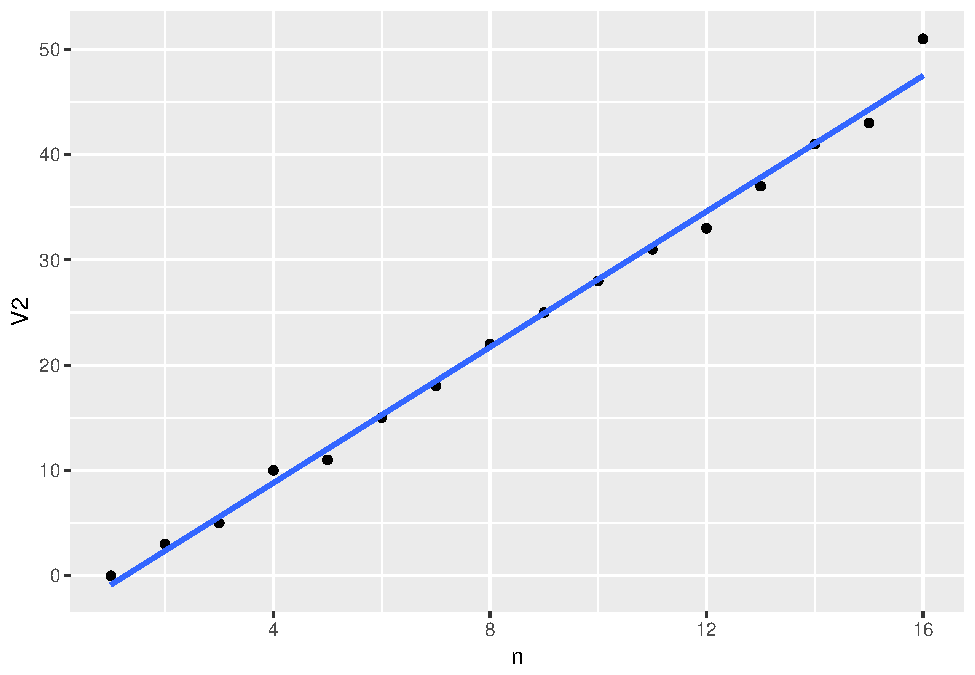
\includegraphics{CHunt_homework1_files/figure-latex/unnamed-chunk-2-1.pdf}

\begin{enumerate}
\def\labelenumi{\alph{enumi}.}
\setcounter{enumi}{1}
\tightlist
\item
  Based on your conclusion in part(a), find a difference equation model
  for the stopping distance data. Test your model by plotting the errors
  in the predicted values against \(n\). Discuss the appropriateness of
  the model.
\end{enumerate}

The plotting of errors shows a linear relationship which will only grow
over time. Therefore, this model is not appropriate.

\[a_{n+1} = 3n+a_n\]

\begin{Shaded}
\begin{Highlighting}[]
\NormalTok{df <-}\StringTok{ }\KeywordTok{as.data.frame}\NormalTok{(}\KeywordTok{cbind}\NormalTok{(n, a_n, }\DataTypeTok{diff =} \KeywordTok{c}\NormalTok{(}\DecValTok{0}\NormalTok{, }\KeywordTok{diff}\NormalTok{(a_n))))}

\NormalTok{for (i in }\DecValTok{1}\NormalTok{:}\KeywordTok{length}\NormalTok{(a_n))\{}
    \NormalTok{if (i ==}\StringTok{ }\DecValTok{1}\NormalTok{)\{}
     \NormalTok{df$a_n2[[i]] <-}\StringTok{ }\NormalTok{a_n[[i]]}
    \NormalTok{\} else \{}
     \NormalTok{df$a_n2[[i]] <-}\StringTok{  }\NormalTok{(df$n[[i]] *(df$diff[}\DecValTok{2}\NormalTok{] -}\StringTok{ }\NormalTok{df$diff[}\DecValTok{1}\NormalTok{]) +}\StringTok{ }\NormalTok{df$a_n2[[i}\DecValTok{-1}\NormalTok{]])    }
    \NormalTok{\}}
\NormalTok{\}}

\KeywordTok{ggplot}\NormalTok{(}\DataTypeTok{data =} \NormalTok{df, }\KeywordTok{aes}\NormalTok{(}\DataTypeTok{x =} \NormalTok{n, }\DataTypeTok{y =} \NormalTok{a_n -}\StringTok{ }\NormalTok{a_n2)) +}\StringTok{ }
\StringTok{        }\KeywordTok{geom_point}\NormalTok{() +}\StringTok{ }
\StringTok{        }\KeywordTok{geom_smooth}\NormalTok{(}\DataTypeTok{method =} \StringTok{"lm"}\NormalTok{, }\DataTypeTok{se =} \OtherTok{FALSE}\NormalTok{)}
\end{Highlighting}
\end{Shaded}

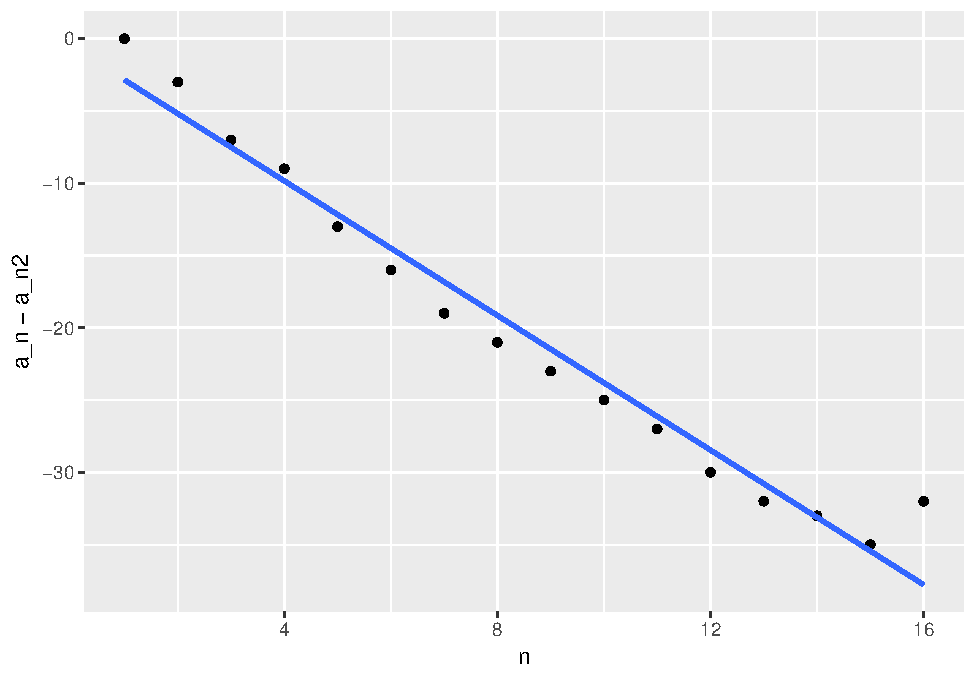
\includegraphics{CHunt_homework1_files/figure-latex/unnamed-chunk-3-1.pdf}
\#\# Page 34: \#13

\subsection{double check this
question}\label{double-check-this-question}

Considering the spreading of a rumor through a company of 1000
employees, all working in the same building. We assume that the
spreading of a rumor is similar to the spreading of a contagious disease
in that the number of people hearing the rumor each day is proportional
to the product of the number who have heard the rumor previously and the
number who have not heard the rumor. This is given by

\[r_{n+1} = r_n + kr_n(1000- _n)\]

where \(k\) is a parameter that depends on how fast the rumor spreads
and \(n\) is the number of days. Assume \(k\) = 0.001 and further assume
that four people initially have heard the rumor. How soon will all 1000
employees have heard the rumor?

\begin{Shaded}
\begin{Highlighting}[]
\NormalTok{r_n <-}\StringTok{ }\DecValTok{4}
\NormalTok{k <-}\StringTok{ }\NormalTok{.}\DecValTok{001}
\NormalTok{count <-}\StringTok{ }\DecValTok{0}

\NormalTok{while (r_n <=}\StringTok{ }\DecValTok{1000}\NormalTok{)\{}
\NormalTok{r_n <-}\StringTok{ }\NormalTok{r_n +}\StringTok{ }\NormalTok{((.}\DecValTok{001}\NormalTok{*r_n)*(}\DecValTok{1000}\NormalTok{-count))}
\NormalTok{count <-}\StringTok{ }\NormalTok{count +}\StringTok{ }\DecValTok{1}
\NormalTok{if (r_n <=}\StringTok{ }\DecValTok{0}\NormalTok{)\{}
  \KeywordTok{print}\NormalTok{(}\StringTok{"no one will have heard the rumor"}\NormalTok{)}
  \NormalTok{break}
 \NormalTok{\}}
\NormalTok{\}}
\end{Highlighting}
\end{Shaded}

\begin{quote}
All 1000 employees will have heard the rumor by the 8 day
\end{quote}

\subsection{Page 55: \#6}\label{page-55-6}

\subsection{TODO finish question}\label{todo-finish-question}

An economist is interested in the variation of the price of a single
product. It is observed that a high price for the product in the market
attracts more suppliers. However, increasing the quantity of the product
supplied tends to drive the price down. Over time, there is an
interaction between price and supply. The economist has proposed the
following model, where \(P_n\) represents the price of the product at
year \(n\), and \(Q_n\) represents quantity. Find the equilibrium values
for the system.

\[P_{n+1} = P_n - 0.1(Q_n -500)\] \[Q_{n+1} = Q_n + .2(P_n - 100)\]
Solve for P \[0 = P-.1(Q - 500)\] \[0 = P-.1Q - 50\] \[P = .1Q -50 \]

Now Solve for Q \[0 = Q + .2(P - 100)\] \[0 = Q +.2p-20\]
\[Q = -.2P+20\]

Substitue and Solve for Value of Q \[Q = -.2(.1Q - 50)+20\]
\[Q = -.02Q + 30\] \[1.02Q = 30\] \[Q = 29.41\] Substitue and Solve for
Value of P \[P = (.1*29.41) -50 \] \[P = -47.06\]

The equilibrium of the systems is P = -47.06; Q = 29.41.

\begin{enumerate}
\def\labelenumi{\alph{enumi}.}
\tightlist
\item
  Does the model make sense intuitively? What is the significance of the
  constants 100 and 500? Explain the significance of the significance of
  the constants -0.1 and 0.2.
\end{enumerate}

The model does not make sense intuitively because the equilibrium has a
negative price, therefore, there must be a price floor that is not
explained in this model where we will no longer sell a product for a
certain price. The significanes of the constants of 100 and 500 is to
reduce the quantity and price for their influence, you'll notice that
-500 is used for quantity which makes sense as our price will vary less
than the quantity so we will want to reduce its impact. The constants of
-0.1 and 0.2 is also to normalize our value, you will notice that the
-.1 is for the price because we expect a decrease in price as the
quantity increase.

\begin{enumerate}
\def\labelenumi{\alph{enumi}.}
\setcounter{enumi}{1}
\tightlist
\item
  Test the initial conditions in the following table and predict the
  long-term behavior
\end{enumerate}

\begin{Shaded}
\begin{Highlighting}[]
\KeywordTok{library}\NormalTok{(knitr)}
\NormalTok{price <-}\StringTok{ }\KeywordTok{c}\NormalTok{(}\DecValTok{100}\NormalTok{, }\DecValTok{200}\NormalTok{, }\DecValTok{100}\NormalTok{, }\DecValTok{100}\NormalTok{)}
\NormalTok{quantity <-}\StringTok{ }\KeywordTok{c}\NormalTok{(}\DecValTok{500}\NormalTok{, }\DecValTok{500}\NormalTok{, }\DecValTok{600}\NormalTok{, }\DecValTok{400}\NormalTok{)}
\NormalTok{row_names <-}\StringTok{ }\KeywordTok{c}\NormalTok{(}\StringTok{"Case A"}\NormalTok{, }\StringTok{"Case B"}\NormalTok{, }\StringTok{"Case C"}\NormalTok{, }\StringTok{"Case D"}\NormalTok{)}
\NormalTok{x <-}\StringTok{ }\KeywordTok{as.data.frame}\NormalTok{(}\KeywordTok{cbind}\NormalTok{(price, quantity))}
\KeywordTok{row.names}\NormalTok{(x) <-}\StringTok{ }\NormalTok{row_names}
\KeywordTok{kable}\NormalTok{(x)}
\end{Highlighting}
\end{Shaded}

\begin{longtable}[]{@{}lrr@{}}
\toprule
& price & quantity\tabularnewline
\midrule
\endhead
Case A & 100 & 500\tabularnewline
Case B & 200 & 500\tabularnewline
Case C & 100 & 600\tabularnewline
Case D & 100 & 400\tabularnewline
\bottomrule
\end{longtable}

\begin{Shaded}
\begin{Highlighting}[]
\KeywordTok{library}\NormalTok{(tidyverse)}
\KeywordTok{library}\NormalTok{(gridExtra)}

\NormalTok{lt_behav <-}\StringTok{ }\NormalTok{function(df)\{}
\NormalTok{for (i in }\DecValTok{1}\NormalTok{:}\DecValTok{149}\NormalTok{)\{}
  \NormalTok{p <-}\StringTok{ }\NormalTok{df$p[[i]] -}\StringTok{ }\NormalTok{.}\DecValTok{1}\NormalTok{*(df$q[[i]] -}\StringTok{ }\DecValTok{500}\NormalTok{)}
  \NormalTok{q <-}\StringTok{ }\NormalTok{df$q[[i]] +}\StringTok{ }\NormalTok{.}\DecValTok{2}\NormalTok{*(df$p[[i]] -}\StringTok{ }\DecValTok{100}\NormalTok{)}
  \NormalTok{result <-}\StringTok{ }\KeywordTok{cbind}\NormalTok{(p, q)}
  \NormalTok{df <-}\StringTok{ }\KeywordTok{rbind}\NormalTok{(df, result)}
  \NormalTok{\}}
\NormalTok{df$count <-}\StringTok{ }\KeywordTok{as.numeric}\NormalTok{(}\KeywordTok{row.names}\NormalTok{(df))}
\NormalTok{df <-}\StringTok{ }\KeywordTok{as.data.frame}\NormalTok{(}\KeywordTok{gather}\NormalTok{(df, count))}
\KeywordTok{colnames}\NormalTok{(df) <-}\StringTok{ }\KeywordTok{c}\NormalTok{(}\StringTok{'count'}\NormalTok{,}\StringTok{'cat'}\NormalTok{,}\StringTok{'value'}\NormalTok{)}
\KeywordTok{return}\NormalTok{(df)}
\NormalTok{\}}

\NormalTok{p <-}\StringTok{ }\NormalTok{x[}\DecValTok{1}\NormalTok{,}\DecValTok{1}\NormalTok{]}
\NormalTok{q <-}\StringTok{ }\NormalTok{x[}\DecValTok{1}\NormalTok{,}\DecValTok{2}\NormalTok{]}
\NormalTok{df <-}\StringTok{ }\KeywordTok{as.data.frame}\NormalTok{(}\KeywordTok{cbind}\NormalTok{(p,q))}
\NormalTok{df}\FloatTok{.1} \NormalTok{<-}\StringTok{ }\KeywordTok{lt_behav}\NormalTok{(df)}

\NormalTok{p <-}\StringTok{ }\NormalTok{x[}\DecValTok{2}\NormalTok{,}\DecValTok{1}\NormalTok{]}
\NormalTok{q <-}\StringTok{ }\NormalTok{x[}\DecValTok{2}\NormalTok{,}\DecValTok{2}\NormalTok{]}
\NormalTok{df <-}\StringTok{ }\KeywordTok{as.data.frame}\NormalTok{(}\KeywordTok{cbind}\NormalTok{(p,q))}
\NormalTok{df}\FloatTok{.2} \NormalTok{<-}\StringTok{ }\KeywordTok{lt_behav}\NormalTok{(df)}

\NormalTok{p <-}\StringTok{ }\NormalTok{x[}\DecValTok{3}\NormalTok{,}\DecValTok{1}\NormalTok{]}
\NormalTok{q <-}\StringTok{ }\NormalTok{x[}\DecValTok{3}\NormalTok{,}\DecValTok{2}\NormalTok{]}
\NormalTok{df <-}\StringTok{ }\KeywordTok{as.data.frame}\NormalTok{(}\KeywordTok{cbind}\NormalTok{(p,q))}
\NormalTok{df}\FloatTok{.3} \NormalTok{<-}\StringTok{ }\KeywordTok{lt_behav}\NormalTok{(df)}

\NormalTok{p <-}\StringTok{ }\NormalTok{x[}\DecValTok{4}\NormalTok{,}\DecValTok{1}\NormalTok{]}
\NormalTok{q <-}\StringTok{ }\NormalTok{x[}\DecValTok{4}\NormalTok{,}\DecValTok{2}\NormalTok{]}
\NormalTok{df <-}\StringTok{ }\KeywordTok{as.data.frame}\NormalTok{(}\KeywordTok{cbind}\NormalTok{(p,q))}
\NormalTok{df}\FloatTok{.4} \NormalTok{<-}\StringTok{ }\KeywordTok{lt_behav}\NormalTok{(df)}


\NormalTok{plot1 <-}\StringTok{ }\KeywordTok{ggplot}\NormalTok{(df}\FloatTok{.1}\NormalTok{) +}\StringTok{ }
\StringTok{         }\KeywordTok{geom_line}\NormalTok{(}\KeywordTok{aes}\NormalTok{(}\DataTypeTok{x =} \NormalTok{count, }\DataTypeTok{y =} \NormalTok{value, }\DataTypeTok{color =} \KeywordTok{as.factor}\NormalTok{(cat))) +}\StringTok{ }
\StringTok{         }\KeywordTok{theme}\NormalTok{(}\DataTypeTok{legend.position=}\StringTok{"top"}\NormalTok{, }\DataTypeTok{legend.direction=}\StringTok{"horizontal"}\NormalTok{, }\DataTypeTok{legend.title=}\KeywordTok{element_blank}\NormalTok{()) }

\NormalTok{plot2 <-}\StringTok{ }\KeywordTok{ggplot}\NormalTok{(df}\FloatTok{.2}\NormalTok{) +}\StringTok{ }
\StringTok{         }\KeywordTok{geom_line}\NormalTok{(}\KeywordTok{aes}\NormalTok{(}\DataTypeTok{x =} \NormalTok{count, }\DataTypeTok{y =} \NormalTok{value, }\DataTypeTok{color =} \KeywordTok{as.factor}\NormalTok{(cat))) +}\StringTok{ }
\StringTok{         }\KeywordTok{theme}\NormalTok{(}\DataTypeTok{legend.position=}\StringTok{"top"}\NormalTok{, }\DataTypeTok{legend.direction=}\StringTok{"horizontal"}\NormalTok{, }\DataTypeTok{legend.title=}\KeywordTok{element_blank}\NormalTok{()) }

\NormalTok{plot3 <-}\StringTok{ }\KeywordTok{ggplot}\NormalTok{(df}\FloatTok{.3}\NormalTok{) +}\StringTok{ }
\StringTok{         }\KeywordTok{geom_line}\NormalTok{(}\KeywordTok{aes}\NormalTok{(}\DataTypeTok{x =} \NormalTok{count, }\DataTypeTok{y =} \NormalTok{value, }\DataTypeTok{color =} \KeywordTok{as.factor}\NormalTok{(cat))) +}\StringTok{ }
\StringTok{         }\KeywordTok{theme}\NormalTok{(}\DataTypeTok{legend.position=}\StringTok{"top"}\NormalTok{, }\DataTypeTok{legend.direction=}\StringTok{"horizontal"}\NormalTok{, }\DataTypeTok{legend.title=}\KeywordTok{element_blank}\NormalTok{()) }

\NormalTok{plot4 <-}\StringTok{ }\KeywordTok{ggplot}\NormalTok{(df}\FloatTok{.4}\NormalTok{) +}\StringTok{ }
\StringTok{         }\KeywordTok{geom_line}\NormalTok{(}\KeywordTok{aes}\NormalTok{(}\DataTypeTok{x =} \NormalTok{count, }\DataTypeTok{y =} \NormalTok{value, }\DataTypeTok{color =} \KeywordTok{as.factor}\NormalTok{(cat))) +}\StringTok{ }
\StringTok{         }\KeywordTok{theme}\NormalTok{(}\DataTypeTok{legend.position=}\StringTok{"top"}\NormalTok{, }\DataTypeTok{legend.direction=}\StringTok{"horizontal"}\NormalTok{, }\DataTypeTok{legend.title=}\KeywordTok{element_blank}\NormalTok{()) }

\KeywordTok{grid.arrange}\NormalTok{(plot1, plot2, plot3, plot4, }\DataTypeTok{ncol=}\DecValTok{2}\NormalTok{)}
\end{Highlighting}
\end{Shaded}

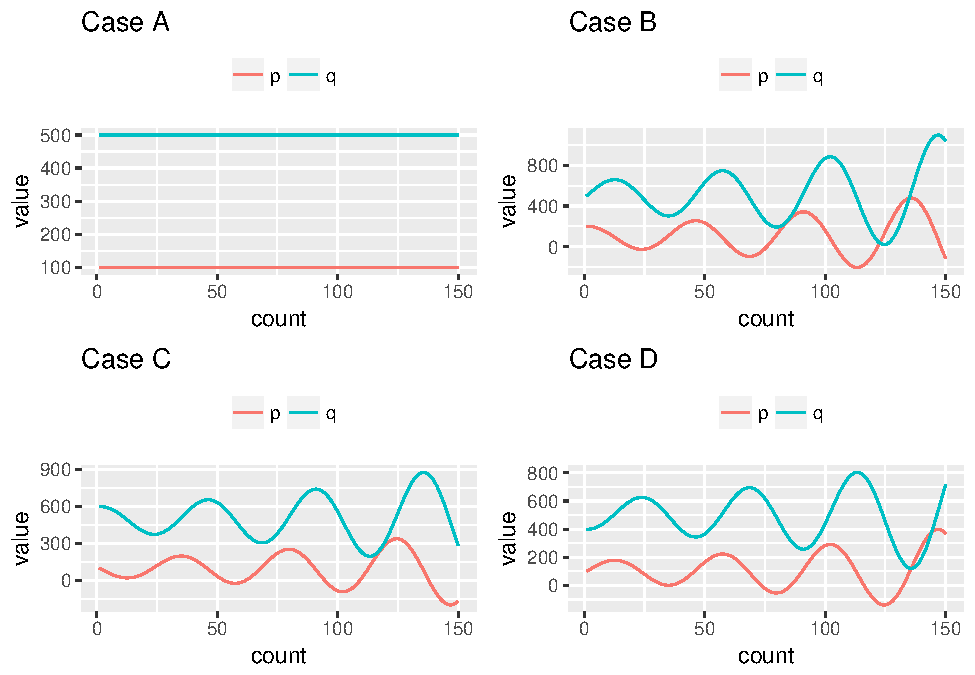
\includegraphics{CHunt_homework1_files/figure-latex/unnamed-chunk-6-1.pdf}


\end{document}
